TensorFlow~\cite{tf} is an open source software library for numerical computation using data flow graphs.
Nodes in these graphs represent mathematical operations, while multidimensional arrays (tensors) move across the edges between them; hence the name.
An example of a computational graph is shown in Figure \ref{fig:comp-graph}.
\begin{figure}[H]
  \centering
  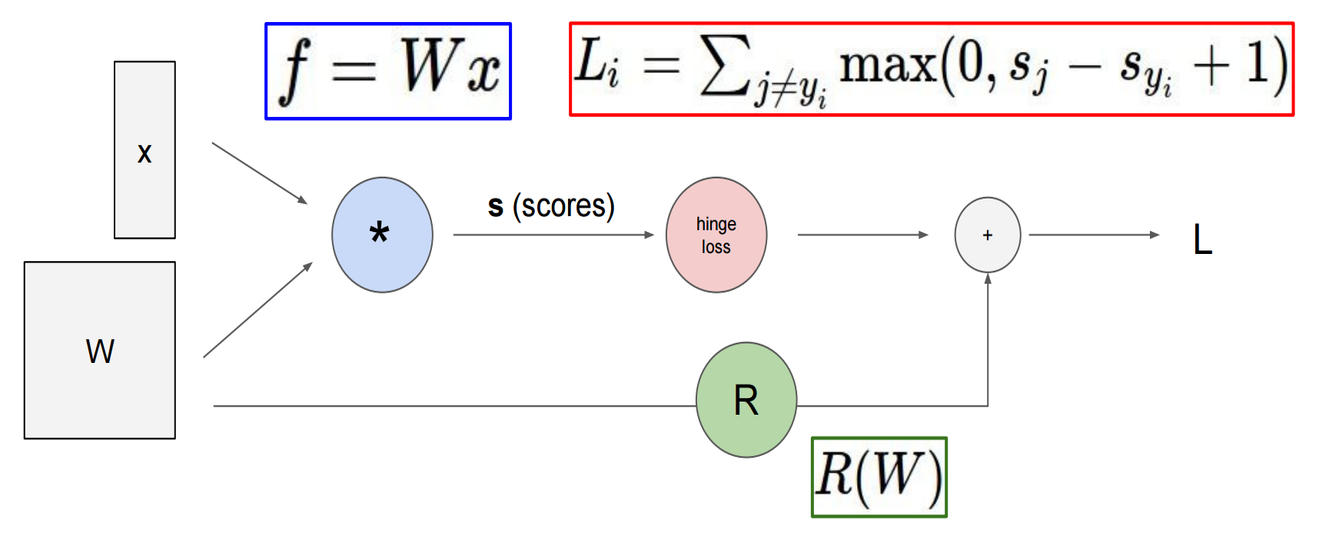
\includegraphics[width=0.8\textwidth]{comp-graph}
  \caption{Computational graph for a regularized Multiclass SVM loss \cite{deepsw}.} 
  \label{fig:comp-graph}
\end{figure}

In TensorFlow, you firstly build the computational graph and then run instances of that graph.
By doing so, the graph is created only once and the framework can apply some optimizations for you before it runs.\\

To make this more concrete, let's consider the linear regression example described in Figure \ref{fig:lin_reg-graph}. 
The corresponding TensorFlow code is shown in Listing \ref{listing:lin-reg}.
\begin{figure}[H]
  \centering
  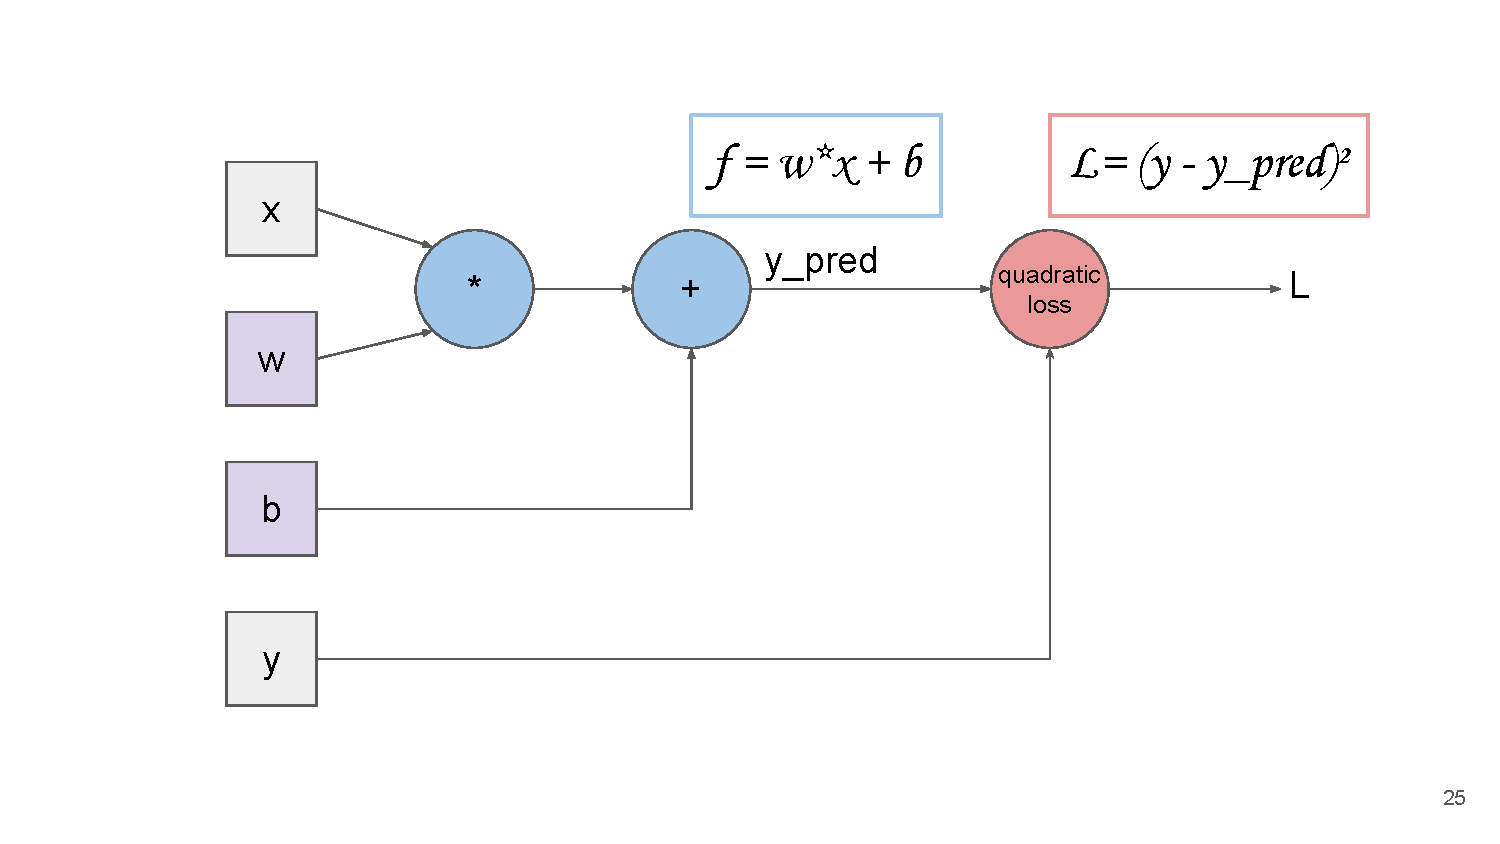
\includegraphics[width=0.75\textwidth, trim={3.5cm 2.2cm 2.2cm 1.8cm}, clip]{simple-graph.pdf}
  \caption{Linear regression computational graph.} 
  \label{fig:lin_reg-graph}
\end{figure}

\lstinputlisting[label=listing:lin-reg, language=Python, caption=Linear regression in TensorFlow., firstline=5,lastline=56]{listings/linear_reg.py}

In the previous snippet, when we build the data flow graph, every variable (such as \texttt{x}, \texttt{w}, \texttt{loss}, and \texttt{train}) is not assigned any value but it is actually an \textit{operation} that is added to the graph.
Specifically, a \texttt{tf.placeholder} represents a container for future values that will be loaded at run time, a \texttt{tf.Variable} instead represents a tensor that will be modified by the learning algorithm during the optimization phase, while the other ones are mathematical operations, as shown in Figure \ref{fig:lin_reg-graph}.\\

We start an execution by opening a \texttt{tf.Session}, to which we pass the graph defined before.
Here, we firstly initialize our \texttt{tf.Variable}s by assigning them their initial value, and then train our model for $\texttt{N\_EPOCHS}$ epochs~\footnote{An epoch is one complete presentation of the training data set to a machine learning model.} by passing each time an input and an output sample via $\texttt{feed\_dict}$ in \texttt{sess.run()}.
\texttt{sess.run()} evaluates the list of operations that are passed in its first argument.
It does so by computing only the nodes in the graph these operations depend on and returns their values at the end of the evaluation.\\

The resulting linear model is shown in Figure \ref{fig:lin_reg-plot}.
\vfill
\begin{figure}[t]
  \centering
  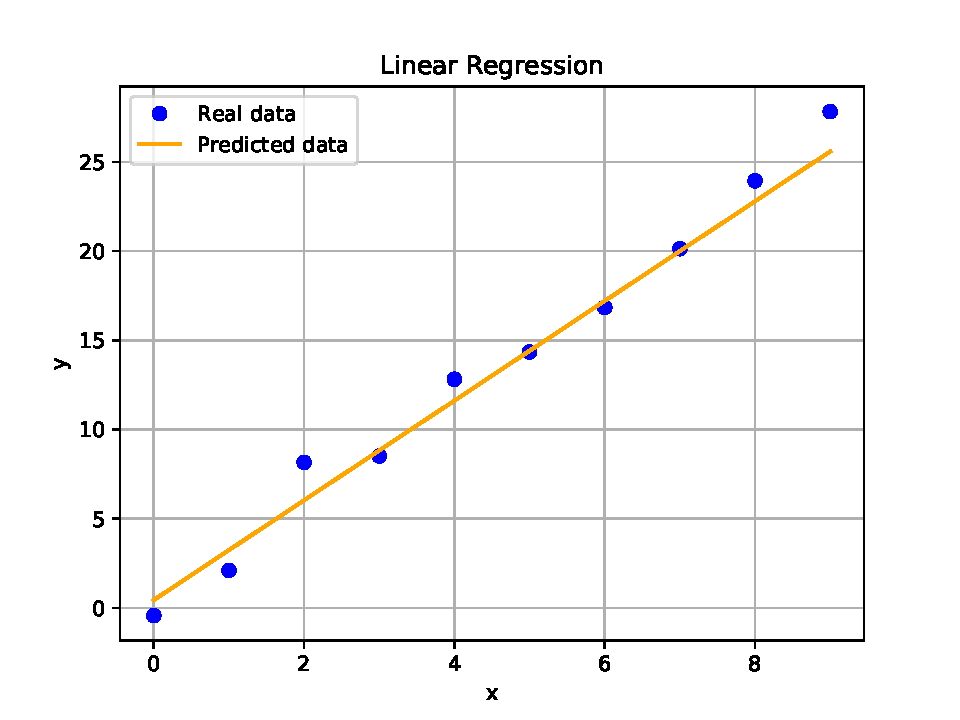
\includegraphics[width=0.7\textwidth,trim={0.5cm 0cm 0cm 0.5cm},clip]{linear_reg.pdf}
  \vspace{-0.5cm}
  \caption{Linear model learned with the example code in Listing \ref{listing:lin-reg}.}
  \label{fig:lin_reg-plot}
\end{figure}

% \begin{mybox}
% 	\begin{center}
% 	\begin{alltt}\tcbfontsize{0.9}
% 	lspci -k | grep -A 3 -i "network"
% 	\end{alltt}
% 	\end{center}
% \end{mybox}
% \noindent


\subsection{Distributed training} \label{sec:tf-dist-th}

As neural networks become larger, it can take weeks to train one of them to achieve the desired accuracy.
It is then of primary importance to distribute the training of these deep neural networks at a massive scale and reduce the training time to hours.\\
TensorFlow offers a large degree of flexibility in the placement of graph operations, allowing easy implementations for parallel computation across multiple workers.\\[-0.2cm]

When splitting the training of a neural network across multiple nodes, the most common strategy is data parallelism, where each node has an instance of the model and reads different training samples.\\
When using TensorFlow, this is achieved with the so-called ``between-graph replication'' setting.
In this context, processes have one of two roles: \textit{Parameter Servers (PS)} or \textit{Workers}.
The former ones host the trainable variables and update them with the values sent by the Workers.
Workers, on the other hand, run the model, send their local gradients to the PSs and receive the updated variables back.\\[-0.2cm]

In doing so, it is essential that all the Workers send their updates of each variable to the same PSs.
To ensure correct device placement of each variable, TensorFlow offers $\texttt{replica\_device\_setter}$, which provides a deterministic method for variable allocation, ensuring that the variables reside on the same devices.\\

Given that each Worker runs the same model, the only high-level changes required in a parallel implementation are the definition of the cluster of nodes and the role of each of them (Parameter Server/Worker).
The following code snippet (from \cite{dist_tf_intro}) shows how to specify such configuration in TensorFlow.
Note that such a script would be executed on each machine in the cluster, but with different arguments.

\begin{lstlisting}[label=listing:tfdist, language=Python, caption=Distributed TensorFlow skeleton.]
import sys
import tensorflow as tf

# Specify the cluster's architecture
cluster = tf.train.ClusterSpec({'ps': ['192.168.1.1:1111'],
                                'worker': ['192.168.1.2:1111',
                                           '192.168.1.3:1111']
                               })

# Parse command-line to specify machine
job_type = sys.argv[1]  # job type: "worker" or "ps"
task_idx = sys.argv[2]  # index job in the worker or ps list
                        # as defined in the ClusterSpec

# Create TensorFlow Server. This is how the machines communicate.
server = tf.train.Server(cluster, job_name=job_type, task_index=task_idx)

# Parameter server is updated by remote clients.
# Will not proceed beyond this if statement.
if job_type == 'ps':
  server.join()
else:
  # Workers only
  with tf.device(tf.train.replica_device_setter(
                      worker_device='/job:worker/task:'+task_idx,
                      cluster=cluster)):
    # Build your model here as if you only were using a single machine

  with tf.Session(server.target):
    # Train your model here
\end{lstlisting}

The first step in running distributed TensorFlow is to define the architecture of the cluster using \texttt{tf.train.ClusterSpec}, where the IP addresses and ports of all the processes for each role are provided.\\
% 
Next, the script determines its job type (or role) and its index among all the processes with the same job type.
This is typically achieved by passing command-line arguments to the script, which are then parsed. 
Here, $\texttt{job\_type}$ specifies whether the node is running a Parameter Server or a Worker task, whereas $\texttt{task\_idx}$ specifies the process's index into its task list. 
An important remark regarding $\texttt{task\_idx}$ is that the list of nodes per role is interpreted as a sorted array.
That is, you cannot arbitrarily set the $\texttt{task\_idx}$ of a given process; instead, this must reflect the position of that process in the original PS or Worker list specified in \texttt{tf.train.ClusterSpec}.
For instance, the script for Worker \texttt{192.168.1.2:1111} must be launched setting its $\texttt{task\_idx}$ to $0$ as it is the first Worker in the list.\\[-0.2cm]

The next step is to use this information to create a TensorFlow Server, which allows this process to communicate with any other server in the same cluster and participate in distributed training.\\[-0.2cm]

If the node is a Parameter Server, it simply joins its threads and waits for them to terminate. 
While it may seem counterintuitive that there is no PS-specific code, the graph elements are actually pushed to it from the workers.\\[-0.2cm]

Conversely, if the device is a Worker, we use $\texttt{replica\_device\_setter}$ to build our model, so that parameters are consistently allocated across our Parameter Servers.
Finally, a \texttt{tf.Session} is created and the model is trained.\\[-0.2cm]

A valuable note is that Parameter Servers and Workers may coexist on the same machine.
This is actually the recommended choice, especially when GPU-enabled nodes are available.
In this case, Parameter Servers would run on CPUs and Workers on GPUs, as their workload is much heavier.
By doing so, not only do we reduce the number of nodes required to run a given application, but also minimize the amount of traffic generated in the network, resulting in higher performance.

\subsubsection{Load Balancing}

In a distributed environment, it is of importance that each Worker has available the updates obtained by the other Workers in order to train faster.
This leads to the need of tackling how to place the variables.\\[-0.2cm]

TensorFlow's \texttt{tf.device} function allows to specify where each operation is stored by means of a device string passed as its argument.
The following snippet of code gives an example of how this is done.
\begin{lstlisting}[label=listing:device-string, language=Python, caption=Variable placement with device strings.]
with tf.device("/job:ps/task:0/cpu:0"):
  weights_1 = tf.get_variable('weights_1', [784, 100])
  biases_1 = tf.get_variable('biases_1', [100])
with tf.device("/job:ps/task:1/cpu:0"):
  weights_2 = tf.get_variable('weights_2', [100, 10])
  biases_2 = tf.get_variable('biases_2', [10])
with tf.device("/job:worker/task:0/gpu:0"):
  # Build your model here
\end{lstlisting}
Here, we ask for $\texttt{weights\_1}$ and $\texttt{biases\_1}$ to be placed in the first PS, while $\texttt{weights\_2}$ and $\texttt{biases\_2}$ in the second one.
Then, each worker designates itself in the third \texttt{with} block in the case of ``between-graph replication''.\\[-0.2cm]

However, it may be difficult to specify where each variable is hosted, especially if many Parameter Servers are desirable for an application in order to distribute the work of updating the variables or distribute the networking load for fetching them to the Workers.
So, TensorFlow allows to pass a device function instead of a device string to \texttt{tf.device}, with the aim of setting a more sophisticated placement strategy.\\[-0.2cm]

Some of such functions are already embedded in TensorFlow.
The simplest of them is called $\texttt{tf.train.replica\_device\_setter}$, which assigns variables to the Parameter Servers in a round-robin fashion as they are created.
A nice property of this device function is that it allows to write all the code to build a model in a single \texttt{with} block.
In fact, this only affects the variables, putting them in different Parameter Servers, while the rest of the operations in the graph go on Workers, simplifying ``between-graph replication'' parallelism.\\[-0.2cm]

The following snippet gives an example of using this function and the resulting variable placement is shown in Figure \ref{fig:loadbalancing-plot} under the round-robin case.
\begin{lstlisting}[label=listing:round-robin, language=Python, caption=Default variable placement with \texttt{replica\_device\_setter}.]
with tf.device(tf.train.replica_device_setter(ps_tasks=3)):
  weights_1 = tf.get_variable('weights_1', [784, 100])
  biases_1 = tf.get_variable('biases_1', [100])
  weights_2 = tf.get_variable('weights_2', [100, 10])
  biases_2 = tf.get_variable('biases_2', [10])
  # Build your model here
\end{lstlisting}
\begin{figure}[H]
  \centering
  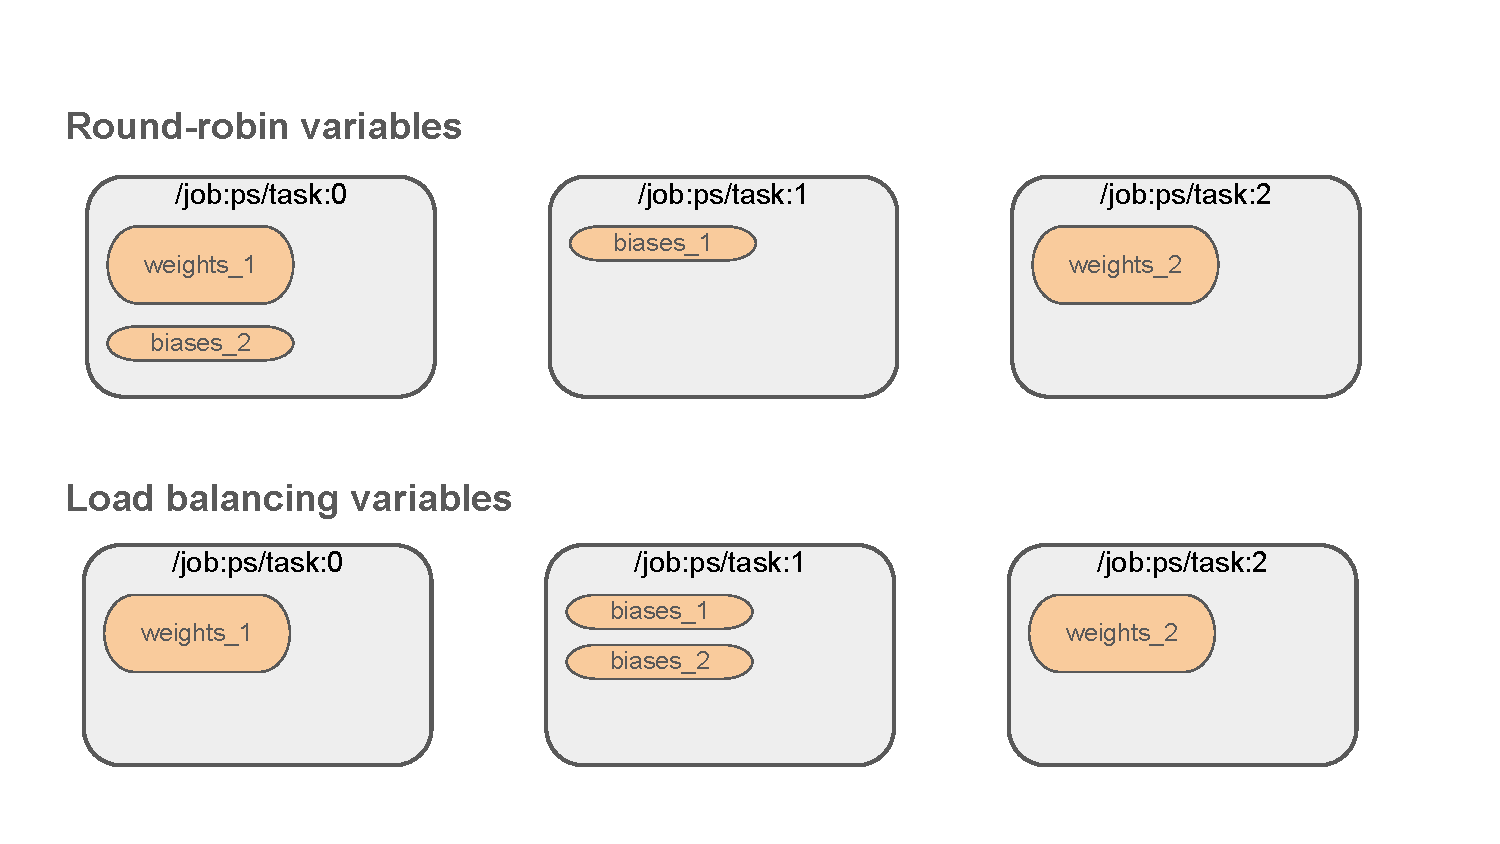
\includegraphics[width=\textwidth,trim={0.5cm 1.2cm 1.5cm 1.7cm},clip]{loadbalancing}
  \vspace{-0.5cm}
  \caption{Round-robin (default) and greedy load balancing variable placement with replica\_device\_setter.} 
  \label{fig:loadbalancing-plot}
\end{figure}
\vspace{-0.3cm}
For this example, Figure \ref{fig:loadbalancing-plot} shows that $\texttt{weights\_1}$ would go to the first Parameter Server, $\texttt{biases\_1}$ would go to the second Parameter Server, $\texttt{weights\_2}$ would be put on the third Parameter Server and $\texttt{biases\_2}$ back on the first Parameter Server.\\
This is obviously not a balance load for these variables, neither in terms of the memory usage nor in terms of the work to be done to update these variables.\\
Moreover, if only two Parameter Servers were used here, we would end up in an even worse case where all the weights would go on the first Parameter Server and all the biases on the second one, giving an even bigger imbalance between these tasks.\\[-0.2cm]

To achieve a more balance load, TensorFlow allows to specify a load balancing strategy in $\texttt{tf.train.replica\_device\_setter}$ as an optional argument.\\
The only one currently available is a simple greedy strategy that does a kind of online bin packing based on the number of bytes of the parameters, giving a more balanced outcome as shown under load balancing variables in Figure \ref{fig:loadbalancing-plot} for our example.
\begin{lstlisting}[label=listing:greedy-loadbalance, language=Python, caption=Greedy load balancing variable placement with \texttt{replica\_device\_setter}.]
greedy =  tf.contrib.training.GreedyLoadBalancingStrategy(...)
with tf.device(tf.train.replica_device_setter(ps_tasks=3, 
                                              ps_strategy=greedy)):
  weights_1 = tf.get_variable('weights_1', [784, 100])
  biases_1 = tf.get_variable('biases_1', [100])
  weights_2 = tf.get_variable('weights_2', [100, 10])
  biases_2 = tf.get_variable('biases_2', [10])
\end{lstlisting}